\section{eo\-G3Replacement$<$ EOT $>$ Class Template Reference}
\label{classeo_g3_replacement}\index{eoG3Replacement@{eoG3Replacement}}
eo\-G3Replacement is an {\bf eo\-Replacement}{\rm (p.\,\pageref{classeo_replacement})}: - no strong elitism (is suppposed to be within a steady-state engine) - choose N (2) parents RANDOMLY - remove them from the parent population - merge offspring and the N removed parents - select best N of this merged population - put them back into parent population  


{\tt \#include $<$eo\-G3Replacement.h$>$}

Inheritance diagram for eo\-G3Replacement$<$ EOT $>$::\begin{figure}[H]
\begin{center}
\leavevmode
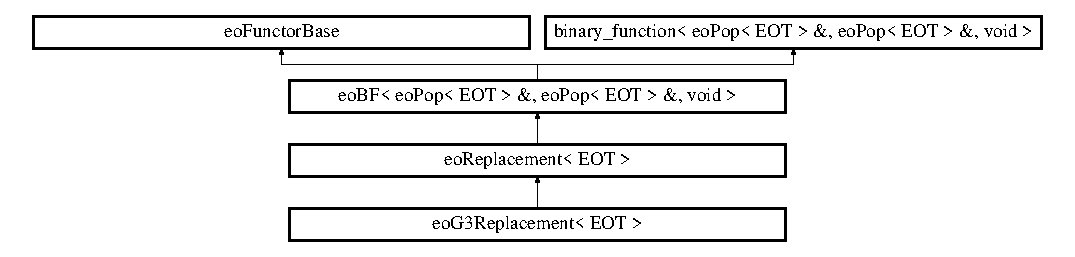
\includegraphics[height=3.01075cm]{classeo_g3_replacement}
\end{center}
\end{figure}
\subsection*{Public Member Functions}
\begin{CompactItemize}
\item 
{\bf eo\-G3Replacement} ({\bf eo\-How\-Many} \_\-how\-Many\-Eliminated\-Parents={\bf eo\-How\-Many}(2, false))\label{classeo_g3_replacement_a0}

\item 
void {\bf operator()} ({\bf eo\-Pop}$<$ {\bf EOT} $>$ \&\_\-parents, {\bf eo\-Pop}$<$ {\bf EOT} $>$ \&\_\-offspring)\label{classeo_g3_replacement_a1}

\begin{CompactList}\small\item\em The pure virtual function that needs to be implemented by the subclass. \item\end{CompactList}\end{CompactItemize}
\subsection*{Private Attributes}
\begin{CompactItemize}
\item 
{\bf eo\-Linear\-Truncate\-Split}$<$ {\bf EOT} $>$ {\bf split}\label{classeo_g3_replacement_r0}

\item 
{\bf eo\-Truncate\-Split}$<$ {\bf EOT} $>$ {\bf reduce}\label{classeo_g3_replacement_r1}

\item 
{\bf eo\-Plus}$<$ {\bf EOT} $>$ {\bf plus}\label{classeo_g3_replacement_r2}

\end{CompactItemize}


\subsection{Detailed Description}
\subsubsection*{template$<$class EOT$>$ class eo\-G3Replacement$<$ EOT $>$}

eo\-G3Replacement is an {\bf eo\-Replacement}{\rm (p.\,\pageref{classeo_replacement})}: - no strong elitism (is suppposed to be within a steady-state engine) - choose N (2) parents RANDOMLY - remove them from the parent population - merge offspring and the N removed parents - select best N of this merged population - put them back into parent population 



Definition at line 50 of file eo\-G3Replacement.h.

The documentation for this class was generated from the following file:\begin{CompactItemize}
\item 
eo\-G3Replacement.h\end{CompactItemize}
